\documentclass[../main.tex]{subfiles}
\begin{document}

\chapter{Integrative approaches for large-scale transcriptome-wide 
association studies}
\labch{gusev2016}

\extauth{Alexander Gusev, Arthur Ko, Huwenbo Shi, Gaurav Bhatia, Wonil 
Chung, Brenda W J H Penninx, Rick Jansen, Eco J C de Geus, Dorret I 
Boomsma, Fred A Wright, Patrick F Sullivan, Elina Nikkola, Marcus 
Alvarez, Mete Civelek, Aldons J Lusis, Terho Lehtimäki, Emma Raitoharju, 
Mika Kähönen, Ilkka Seppälä, Olli T Raitakari, Johanna Kuusisto, Markku 
Laakso, Alkes L Price, Päivi Pajukanta \& Bogdan Pasaniuc; Nature 
Genetics 2016}

\begin{external_abstract}{title=\textit{Abstract}}
Many genetic variants influence complex traits by modulating gene 
expression, thus altering the abundance of one or multiple proteins. 
Here we introduce a powerful strategy that integrates gene expression 
measurements with summary association statistics from large-scale 
genome-wide association studies (GWAS) to identify genes whose 
cis-regulated expression is associated with complex traits. We leverage 
expression imputation from genetic data to perform a transcriptome-wide 
association study (TWAS) to identify significant expression-trait 
associations. We applied our approaches to expression data from blood 
and adipose tissue measured in \char`\~3,000 individuals overall. We 
imputed gene expression into GWAS data from over 900,000 phenotype 
measurements to identify 69 new genes significantly associated with 
obesity-related traits (BMI, lipids and height). Many of these genes are 
associated with relevant phenotypes in the Hybrid Mouse Diversity Panel. 
Our results showcase the power of integrating genotype, gene expression 
and phenotype to gain insights into the genetic basis of complex traits.
\end{external_abstract}

\section{Introduction}

As we have said, the \textit{rationale} that lies behind the association 
of gene expression to phenotype is that many genetic variants influence 
traits by altering the regulation of the expression of some genes. 
PrediXcan, with which we dealt in the previous section, is not the only 
method to perform a TWAS. In particular, in 2016 it has been proposed a 
new approach where individual-level data are superfluous: only summary 
association statistics\sidenote{By summary association statistics we 
mean the effect size of all the SNPs and, optionally, the summary 
linkage disequilibrium information for the samples (\ie the pairwise LD 
among typed SNPs). The genotype of single individuals is unknown.} from 
a GWAS is needed. This is an important advantage since, normally, only 
the summary-level data of a study are publicly available due to privacy 
concerns.

The description of this new approach is as follows. First, a Bayesian 
sparse mixed regression model finds the correlation between each SNP and 
gene expression from a reference transcriptome data set, and accordingly 
assigns a weight to each SNP; next, starting from the summary 
association score of a genotyped SNP with the disease status, and from 
the weight by which the SNP alters gene expression, the association 
between expression and disease status can be estimated. Furthermore, by 
considering the linkage disequilibrium between the genotyped SNP and a 
non-genotyped SNP, and the weight by which the non-genotyped SNP alters 
expression, the association between expression of non-genotyped SNPs and 
disease status can be \enquote{imputed}. The approach is quite different 
from PrediXcan, especially in the second part (\reffig{gusev2016/1}).

\begin{figure}
	\centering
	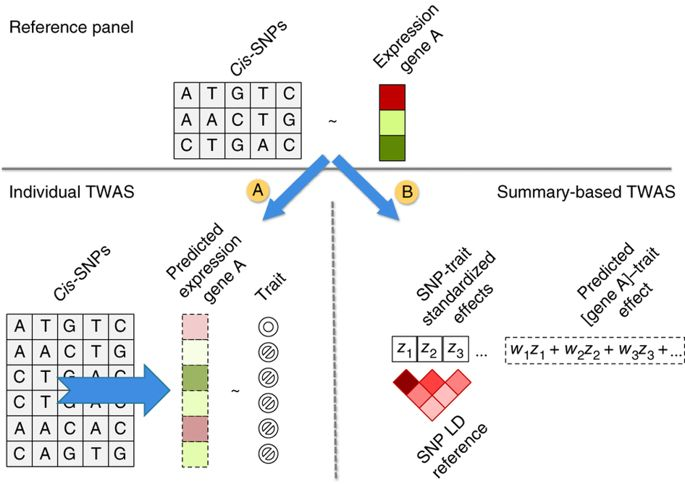
\includegraphics{gusev2016/1-TWAS_schematic}
	\caption{Schematics and comparison of individual-level and 
summary-level TWAS.}
	\labfig{gusev2016/1}
\end{figure}

There are some relevant points in this new method: its being based on 
summary association statistics greatly increases the effective sample 
size, for the method can in principle be applied to any GWA study; 
moreover, the authors emphasise the specificity of their approach, for 
its focus is on the genetic component of expression only, computed from 
a reference transcriptome data set of healthy individuals; therefore, it 
is guaranteed that, save for pleiotropic effects\sidenote{Pleiotropy is 
a phenomenon where a single genetic locus \textit{independently} 
influences more than one phenotype; for instance, an allele could alter 
gene expression on the one hand, and lead to a disease through a 
different mechanism. Pleiotropic effects cannot be modeled by TWAS.}, if 
an association between expression and trait is detected, it is 
ultimately due to genetic factors. In general, the TWAS approach is not 
able to detect associations between gene and disease if the mechanism 
does not involve a change in gene expression. Several are the ways in 
which genomic variation can be related to gene expression and phenotypic 
variation (\reffig{gusev2016/2}). Transcriptome-wide association studies 
work only under the hypothesis that a genetic variant influences, 
directly or indirectly, the phenotype through gene expression.

\begin{figure}
	\centering
	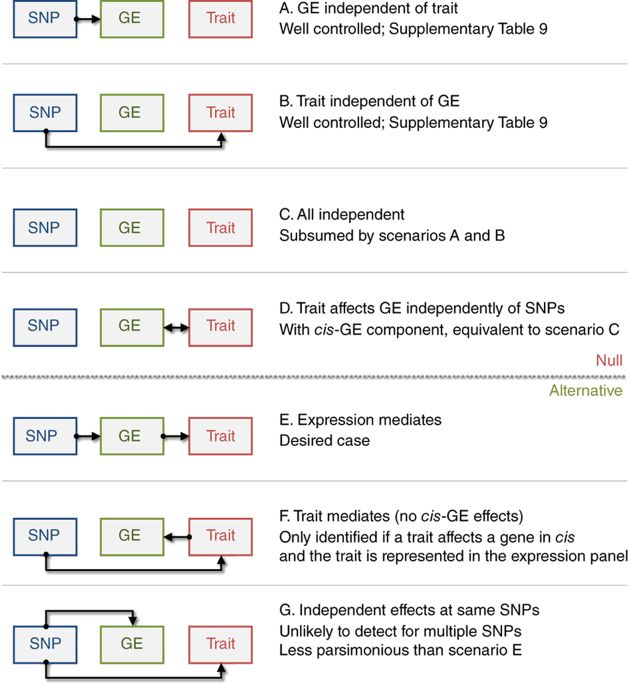
\includegraphics[width=0.8\textwidth]{gusev2016/2-causality_models}
	\caption{The possible models of causality. TWAS are useless in cases 
A-D, but work for E-G.}
	\labfig{gusev2016/2}
\end{figure}

The models to find the coefficients by which each SNP alters gene 
expression were trained on about 3,000 individuals whose expression data 
from blood and adipose tissues, as well as genotype data, were 
available. With the help of a simulated dataset, they compared their 
approch with others previously proposed, showing that theirs is a 
significant improvement. Moreover, they reanalysed an existing dataset 
of a small-cohort lipid GWAS, finding that most of the novel 
associations they obtained with the TWAS had been reported in a 
larger-cohort GWAS, and implying that their method is statistically more 
powerful than SNP-based approaches, especially when the sample size is 
small. Finally, they applied their method to GWAS data for over 900,000 
phenotype measurements, identifying many new disease-associated genes.

\reftab{comparison} illustrates the differences between the Gamazon and 
the Gusev methods.

\begin{table}
	\centering
	\begin{tabular}{ l c c }
		\toprule
		& PrediXcan & Integrative \\
		\midrule
		Training data sets & DGR & METSIM, YFS, NTR \\
		Prediction of expression & elastic net & BSLMM \\
		Input data & individual level & summary level \\
		Gene-disease association & logistic regression & correlation \\
		\bottomrule
	\end{tabular}
	\caption{Comparison between PrediXcan and the integrative approach.}
	\labtab{comparison}
\end{table}

\section{Estimation of SNP-expression weights}

The accuracy of the prediction of a gene's expression cannot be greater 
than the heritability of the expression of that gene itself (see the 
discussion in \refsec{heritability}). For example, if a quantitative 
trait is normally-distributed in a population, but every individual has 
the same alleles at the same trait-associated loci, the genetic variance 
in that population will be $0$, and the heritability for such a trait 
would consequently be $0$ as well. In such circumstances, it is not 
possible to predict the trait using the \cis-genetic component of gene 
expression, for there is no such component: the differences in the 
individuals' traits depend only upon the environment, and it is 
notoriously difficult to quantitatively measure the effect of 
environment, especially outside of the laboratory. On the other hand, if 
the trait has an $h^2$ of 1, its manifestation can be predicted from the 
genotype with arbitrary accuracy, save for random variation due to 
chance\sidenote{Indeed, environment and chance have different effects: 
the former generates a systematic bias in the trait, but is difficult to 
quantitfy, while the latter alters the trait because of the stochastic 
nature of life, and its average effect is zero in a large enough 
population.}.

In order to predict a quantitative trait from the genotype of the 
individuals, samples for which both gene expression and genotype data 
are present are necessary. The authors collected about 3,000 samples 
from three data sets: METSIM, YFS and NTR. Both the quantitative 
measures of the phenotypes and the gene expression levels were 
normalised and standardised before the analysis.

\marginnote{
\begin{description}
	\item[YFS] is a long-term study of cardiovascular diseases in young 
finns.
	\item[METSIM] studied the metabolic syndrome in men, collecting 
adipose tissue data in follow-ups of the young finns study.
	\item[NTR] measured gene expression in peripheral blood in more than 
2000 twins, computing the heritability of genes and finding 
	 eQTL.
\end{description}
}

From the data obtained from the about 3,000 individuals, the 
heritability of the expression of each gene was computed 
(\reffig{gusev2016/S1}) using the tool GCTA\autocite{Yang2011a}. For 
each gene, two heritability measures were estimated: \cis- and \trans- 
heritability, labelled $h_{g,cis}^2$ and $h_{g,trans}^2$; 
\cis-heritability refers to the proportion of variance in gene 
expression that is imputable to variance in loci up to 1Mb from the 
gene, whereas \trans-heritability is the proportion of variance in gene 
expression explained by the rest of the loci. Since on average any two 
non-related individuals differ at 0.1\% of loci \autocite{Auton2015}, in 
order to estimate \trans variance a very large sample size is needed, 
far larger than the 3,000 individuals used in this study, and this is 
the reason why estimates of \trans-heritability are close to $0$. All 
subsequent analysis were based on the 6,924 \cis-heritable genes 
(\reffig{gusev2016/3}). Restricting the analysis to \cis-SNPs greatly 
increases the statistical power of the study, for the number of 
predictors of gene expression becomes quite small; as previously 
explained, the multiple testing burden is also decreased.

\begin{figure}
	\centering
	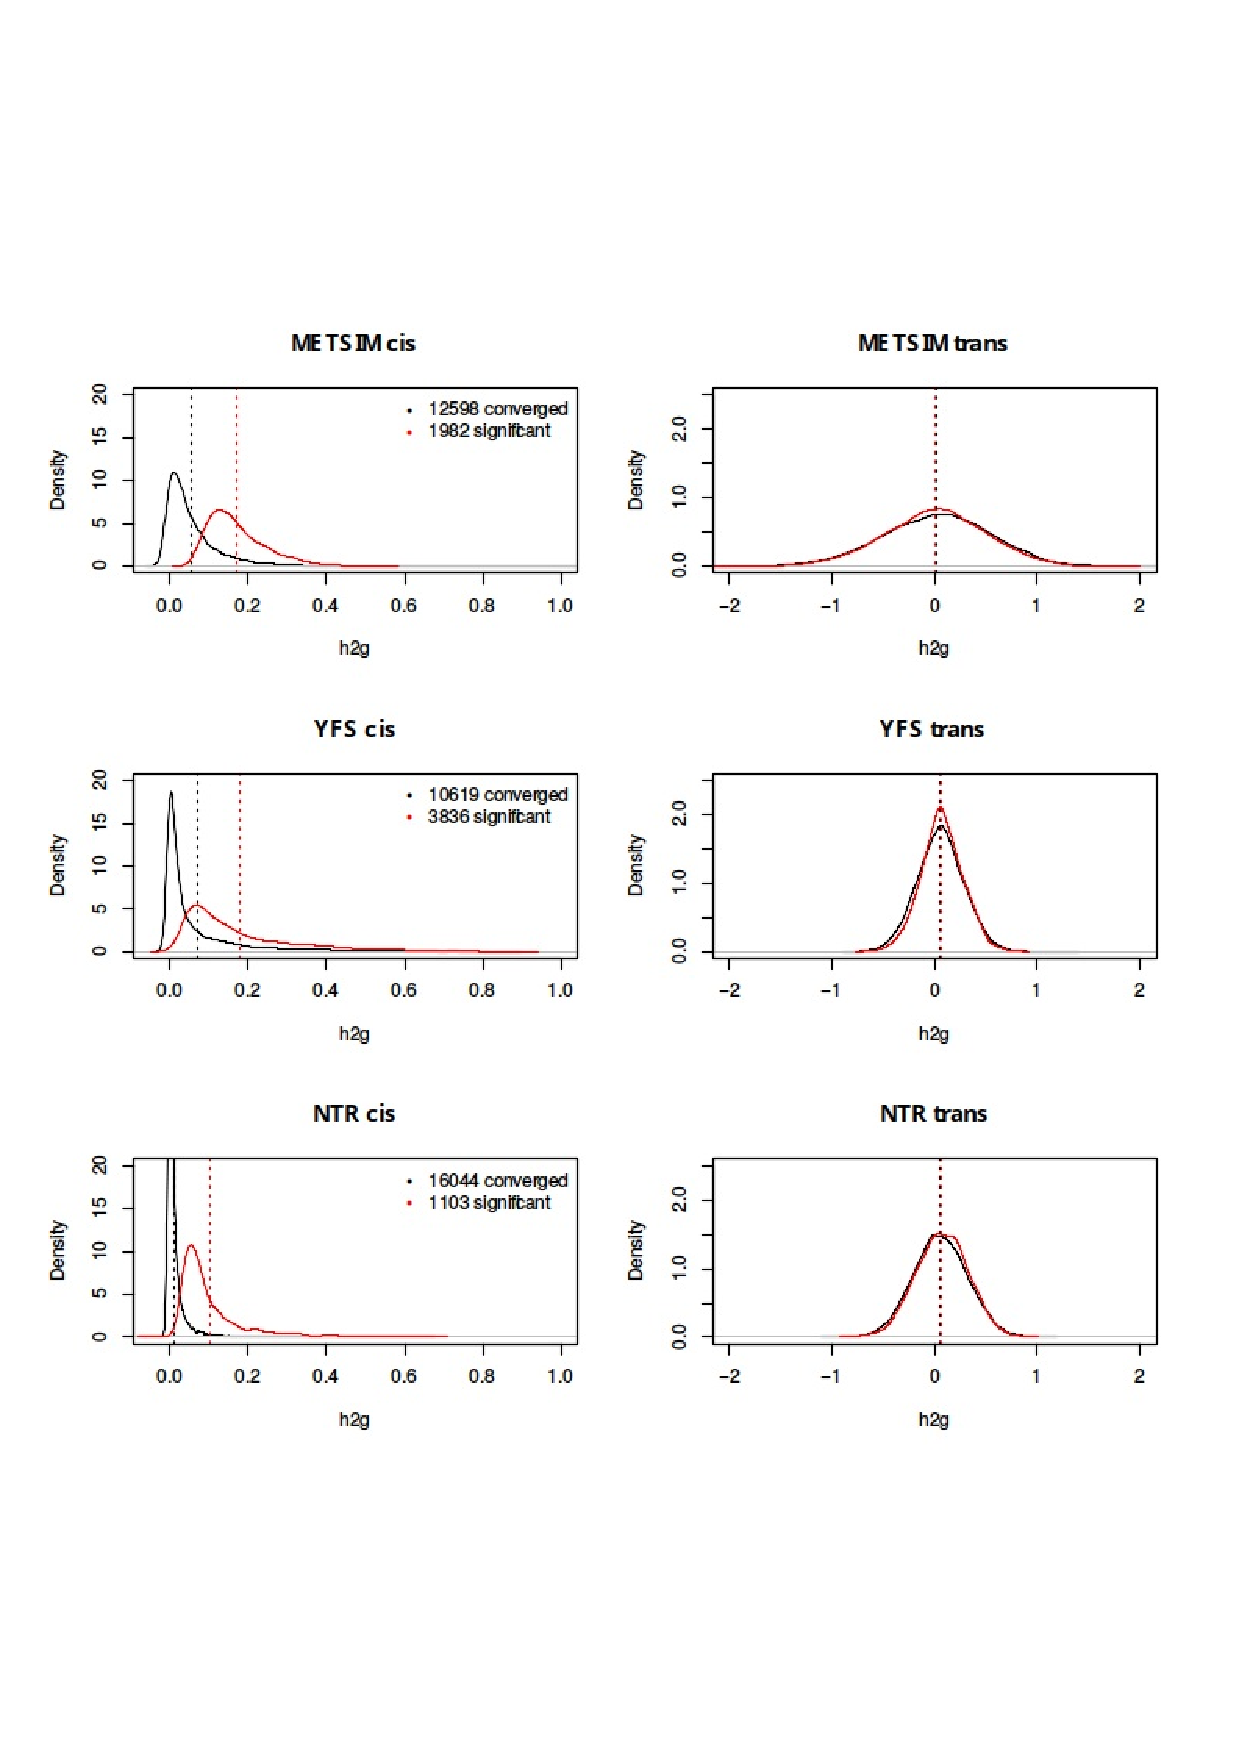
\includegraphics{gusev2016/S1-heritability_distribution}
	\caption{Heritability distribution in the METSIM data set. 
		Distributions in the other data sets are not reported.}
	\labfig{gusev2016/S1}
\end{figure}

\begin{figure}
	\centering
	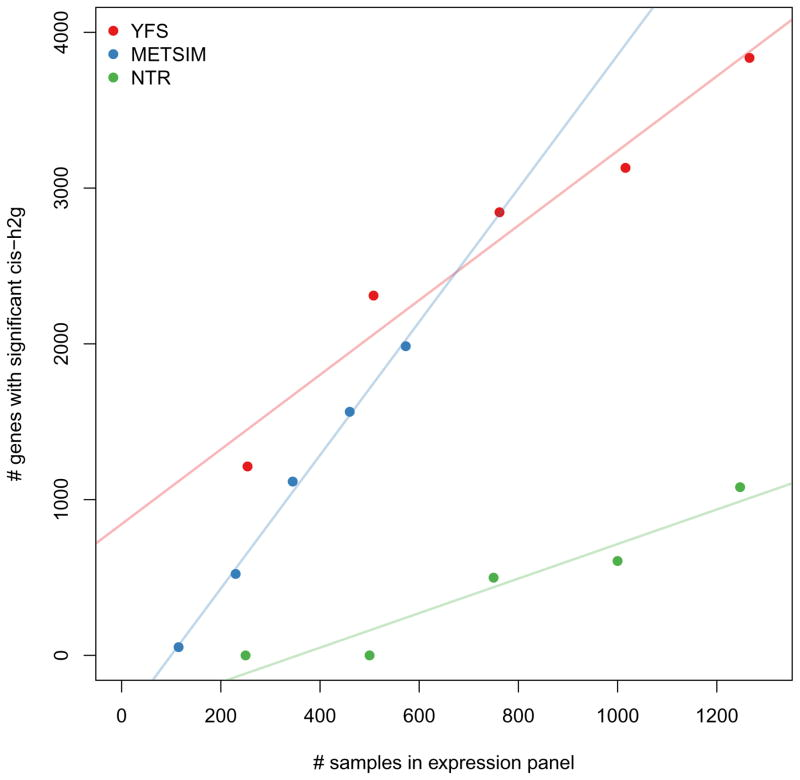
\includegraphics[width=0.7\textwidth]{gusev2016/3-heritable_genes}
	\caption{The 6,924 heritable genes, distributed according to their 
origin}
	\labfig{gusev2016/3}
\end{figure}

Having computed heritability, a statistical model could be trained to 
predict gene expression from genotype data; this is only needed to 
estimate the weights of which each SNP alters gene expression. Two 
different models, all based on the \cis-SNPs, were employed: the first 
was a best linear unbiased model (BLUP) and the second a Bayesian sparse 
linear mixed model (BSLMM, see \refsec{regression} for technical 
details). The performance of each model was evaluated by 
cross-validation. Moreover, these two models were compared to the 
predictions of gene expression made from the best \cis-eQTL. The 
Bayesian model was the best one (\reffig{gusev2016/4}), therefore it was 
used for subsequent analysis.

\begin{figure}
	\centering
	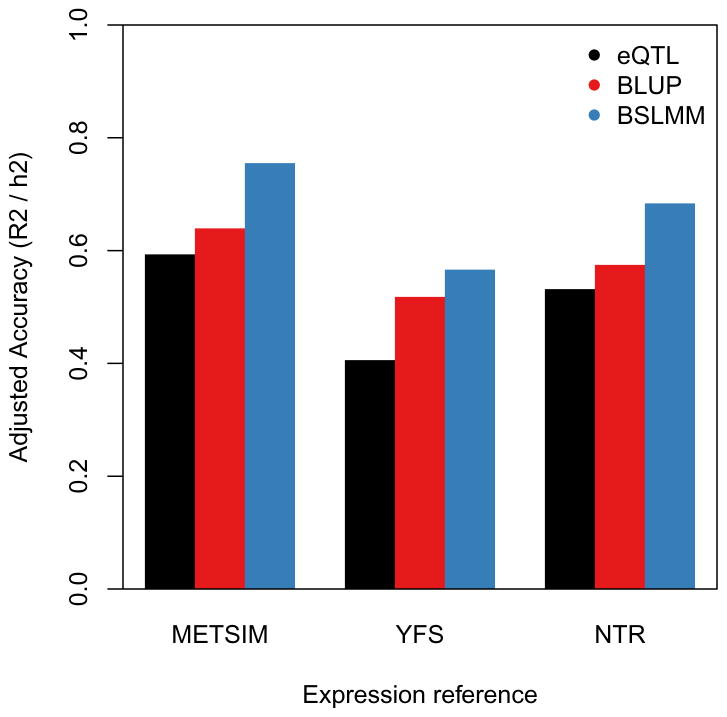
\includegraphics[width=0.75\textwidth]{gusev2016/4-prediction_accuracy_comparison}
	\caption{BSLMM performs better, as can be seen by the 
		cross-validation results.}
	\labfig{gusev2016/4}
\end{figure}

\section{Application to a small-cohort GWAS}

The BSLMM was trained on the three data sets (METSIM, YFS and NTR) as 
described previously, and the weight of each SNP was estimated; then, 
the correlations between the \cis-regulated expression of each gene and 
the lipid phenotypes from the GWAS were calculated using summary-level 
statistics. 25 correlations were found between phenotype and genes that 
were more than 500 kb far from any significant SNP in that study, and 19 
of these genes contained at least a significant SNP in a larger blood 
lipid GWAS. This result is an additional confirmation that the proposed 
method is valid.

The method they used to find associations between gene expression and 
phenotype from the summary statistics of the GWAS is a generalisation of 
a method previously proposed by the same authors to impute SNP-phenotype 
associations in a GWAS, knowing only the association score of genotyped 
SNPs\autocite{Pasaniuc2014} and optionally the summary LD statistics. In 
essence, the original method is based on the assumption that the 
z-scores\sidenote{The z-score is the standardised association score and 
	measures of how many standard deviations the score differs from the 
mean.} of the SNPs in a locus are normally-distributed, with mean $0$ if 
there is no association, and with a standard deviation depending on the 
correlation among the SNPs, that is, on the LD structure of the locus. 
The LD structure can be taken from the reference genome or, if 
available, directly from the population of the GWAS. Thus, with the 
previously developed method, by knowing the z-score of a genotyped SNP 
and the LD between a non-genotyped SNP and the genotyped one, it is 
possible to estimate the z-score of the non-genotyped SNP. The method 
was adapted in this paper so as to wheight the imputed z-score of a SNP 
by the coefficient of which that SNP alters gene expression. This 
coefficient was previously estimated in a reference transcriptome data 
set using the BSLMM.

In other words, the association score for a gene can be expressed as

\begin{equation}
	\label{eq:summary_twas}
	\mathbf{Z}_{TWAS} = \frac{\mathbf{W} \mathbf{Z}_{GWAS}}
		{\sqrt{\mathbf{W} \mathbf{D} \mathbf{W}^t}}\,,
\end{equation}

where $\mathbf{Z}$ is a vector of the standardised effect sizes of the 
\cis SNPs of one gene; $\mathbf{W}$ is a vector of the weights of those 
SNPs; $\mathbf{D}$ is the linkage disequilibrium matrix, representing 
the correlation between SNPs. Therefore, the numerator is a linear 
combination of effect sizes and weights: $w_1 z_1 + w_2 z_2 + \ldots$, 
while the denominator is the standard deviation of the numerator.

\section{Application to 900,000 phenotypes}

One of the most innovative features of this approach is its broad 
applicability. Indeed, its potential was unleashed on three GWAS which 
accounted for over 900,000 phenotype measurements of obesity-related 
traits\sidenote{Lipid measures (high-density lipoproteins [HDL] 
cholesterol, low-density lipoprotein [LDL] cholesterol, total 
cholesterol [TC], and triglycerides [TG]); height; and BMI}. 665 
significant gene-trait associations were found, 69 of which genes did 
not overlap any SNP which was reported by the original GWA studies.

Those 69 novel associations are the most interesting ones, therefore 
they were the focus of a functional analysis: on the one hand, their 
presence was sought in the Hybrid Mouse Diversity Panel (HMDP), which 
collects obesity-related phenotypes; on the other hand, tissue-specific 
enrichments of these genes was evaluated. Many of the 69 genes were 
indeed present and they were associated with an obesity-related trait. 
Moreover, the tissue enrichment analysis, performed with DEPICT, showed 
that the novel genes were specific of hypothalamus and neurosecretory 
systems, which is consistent with recent discoveries on obesity. No 
pathway enrichment analysis was performed.

\section{Allelic heterogeneity}
\labsec{allelic_heterogeneity}

For comparison purposes, the authors built an array of simulated data 
sets, each modelling a possible scenario (1 causal variant, 5\% causal 
or 10\% causal), and performed a TWAS, a GWAS and an eGWAS\sidenote{In 
the GWAS, trait-associated variants falling in a gene are retained; in 
the eGWAS, only the best eQTL for each gene is tested for associations 
with the trait.} on them. On the whole, the performance of the TWAS was 
comparable to the others when the number of causal variants was small, 
but it was better at associating multiple causal variants to the trait 
(\reffig{gusev2016/5}).

\begin{figure}
	\centering
	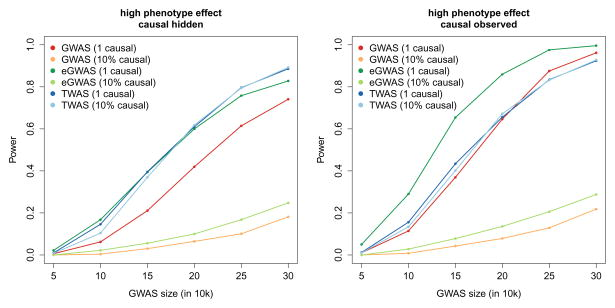
\includegraphics{gusev2016/5-association_power}
	\caption{The TWAS approach compared to GWAS and eGWAS.}
	\labfig{gusev2016/5}
\end{figure}

This can be explained by allelic heterogeneity, \ie the presence of 
multiple different variants affecting the same gene in the same way. For 
instance, $\beta$-thalassemia can be due to several mutations. In these 
cases, GWAS are disadvantages because they focus on single variants, 
each of which can be very rare. On the other hand, whatever genetic 
variant is present, the expression of the involved gene will be altered 
in nearly the same way.

\section{Discussion}

The main idea introduced with this work, with respect to the previous 
one, is that individual-level data are no longer necessary. In the words 
of the authors, this method can be viewed as \enquote{a test for the 
correlation between the genetic component of expression and the genetic 
component of a trait}. Indeed, the z-score of the association between 
gene expression and trait is a function of the z-scores of the \cis SNPs 
of that gene, the weight of which those SNPs alter the expression of the 
gene, and the linkage disequilibrium between them (see equation 
\eqref{eq:summary_twas}).

This complicates the statistics, as more assumptions are needed (in 
particular, that z-scores are normally distributed with mean $0$ in the 
case of no association), and another downside is that rare variants are 
less likely to be identified. Nevertheless, the benefits outweight the 
costs, for the method can be used on virtually every GWAS performed to 
date, and just in this article many novel genes were found associated to 
phenotypes.

Here, a Bayesian sparse linear mixed model is used instead of elastic 
net; both perform variable selection, meaning that only the best 
predictors are employed. The main difference between the two regression 
models is that the former takes account of random effects, modeled with 
a normal distribution.

Another possible point of debate about this work is that genetic 
variation does not only alter gene expression. A SNP can have effects on 
splicing, transcription start or end site or other RNA editing 
processes, without altering the expression of the gene. The next article 
shall deal with such problems.

\end{document}
